\documentclass[12pt,a4paper]{article}
\usepackage{physics}
\usepackage{amssymb}
\usepackage{subcaption}
\usepackage{colortbl}
\usepackage{musicography}
\newcommand{\activity}{Activity 13 -- Perceptron}
\input{spp.dat}

\begin{document}

\title{\TitleFont \activity}
\author[ ]{\textbf{Kenneth V. Domingo} \\
2015--03116 \\
App Physics 186, 1\textsuperscript{st} Semester, A.Y. 2019--20}
\affil[ ]{\corremail{kvdomingo@up.edu.ph} }

\maketitle
\thispagestyle{titlestyle}

\section*{Results and Discussion}
\setcounter{section}{1}

For this activity \cite{soriano}, I used the features extracted from the fruits (50 each of apples, mangoes, bananas) from the previous activity. The feature space in $a^*$-$b^*$ (obtained from the $L^*a^*b^*$ color space) is shown in Fig. \ref{fig:ab-space}. Since we'll be working with a linear classifier for now, we need to process only two classes at a time. We design the perceptron so that it follows a simple weight update rule

\begin{equation}\label{eq:weight-update}
	\Delta w_j = \eta \qty(y^i - z^i)x_j^i
\end{equation}

\noindent where $y$ is the ground truth label, $z$ is the predicted label, and $\eta$ is the learning rate, which we set to 0.01. The perceptron is trained for 100 epochs and the decision boundary is obtained from the final weights. The decision boundary and decision contours for each class pair is shown in Fig. \ref{fig:boundaries}.

\begin{figure}[htb]
	\centering
	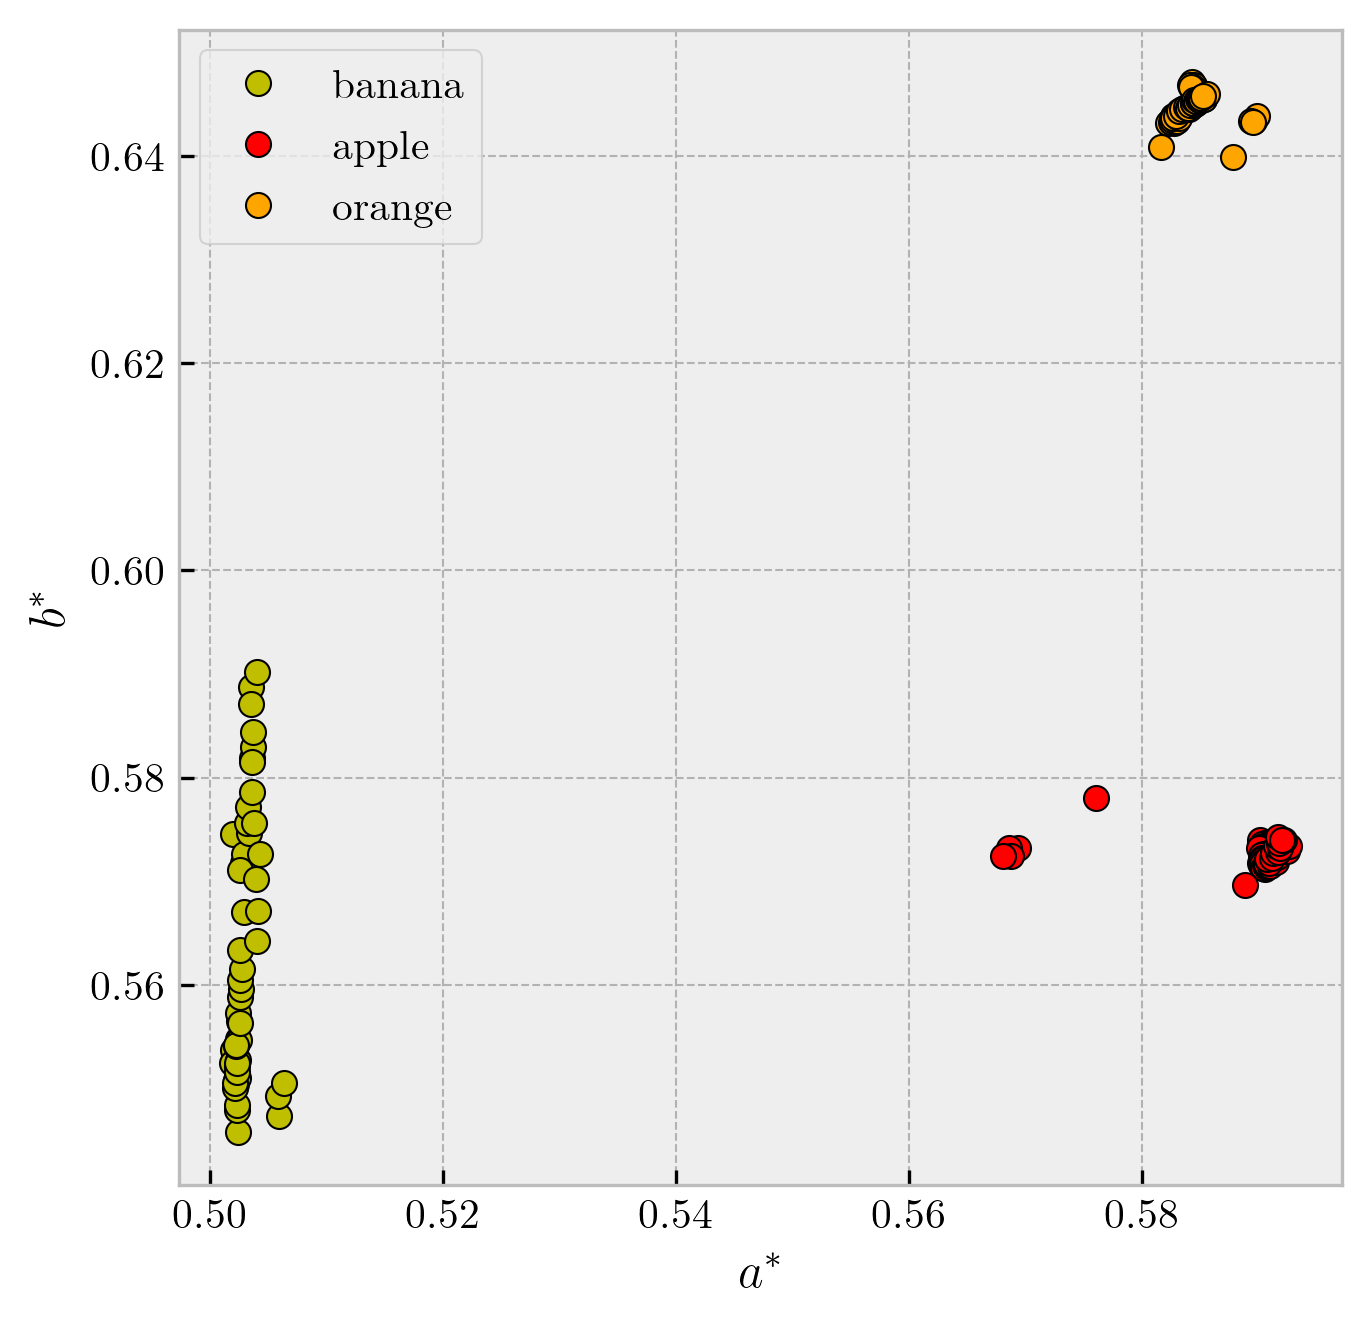
\includegraphics[width=0.6\textwidth]{ab-space.png}
	\caption{Feature space in $a^*$-$b^*$.}
	\label{fig:ab-space}
\end{figure}

\begin{figure}[htb]
	\centering
	\begin{subfigure}[h!]{0.3\textwidth}
		\centering
		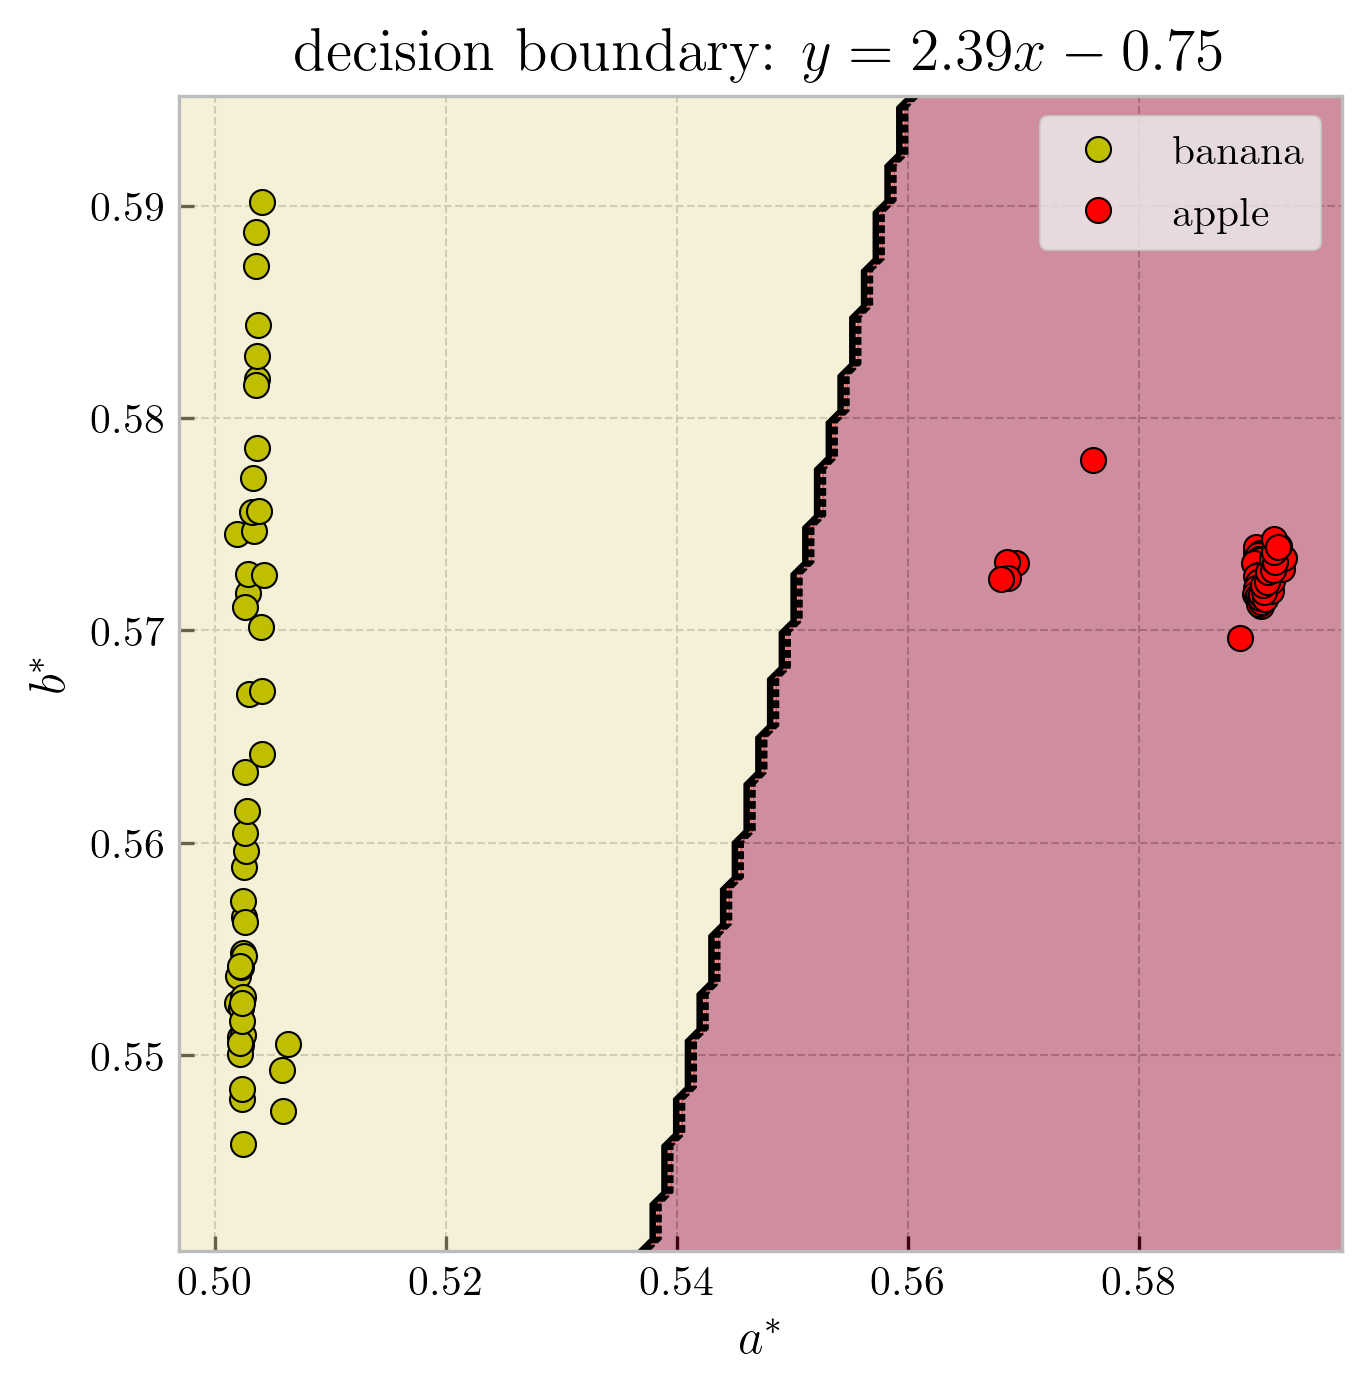
\includegraphics[width=\textwidth]{ban-app_decision.png}
		\caption{banana-apple}
		\label{fig:banana-apple}
	\end{subfigure}
	\begin{subfigure}[h!]{0.3\textwidth}
		\centering
		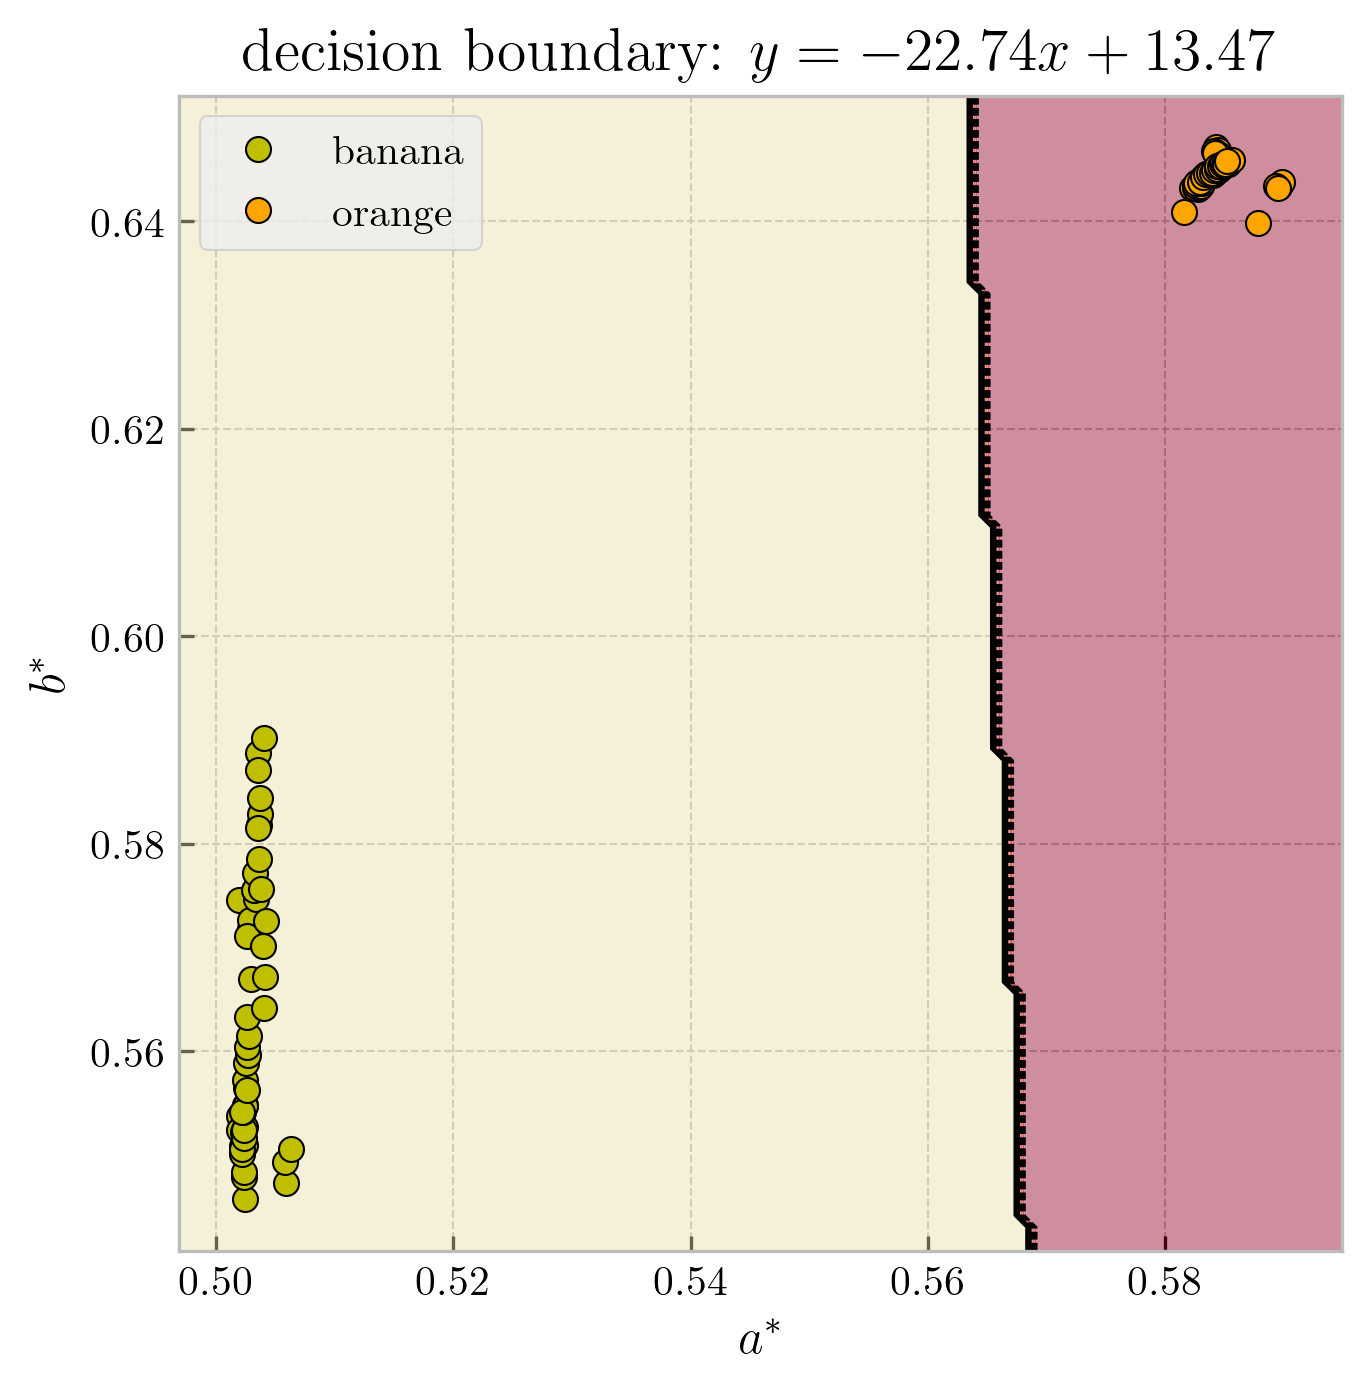
\includegraphics[width=\textwidth]{ban-ora_decision.png}
		\caption{banana-orange}
		\label{fig:banana-orange}
	\end{subfigure}
	\begin{subfigure}[h!]{0.3\textwidth}
		\centering
		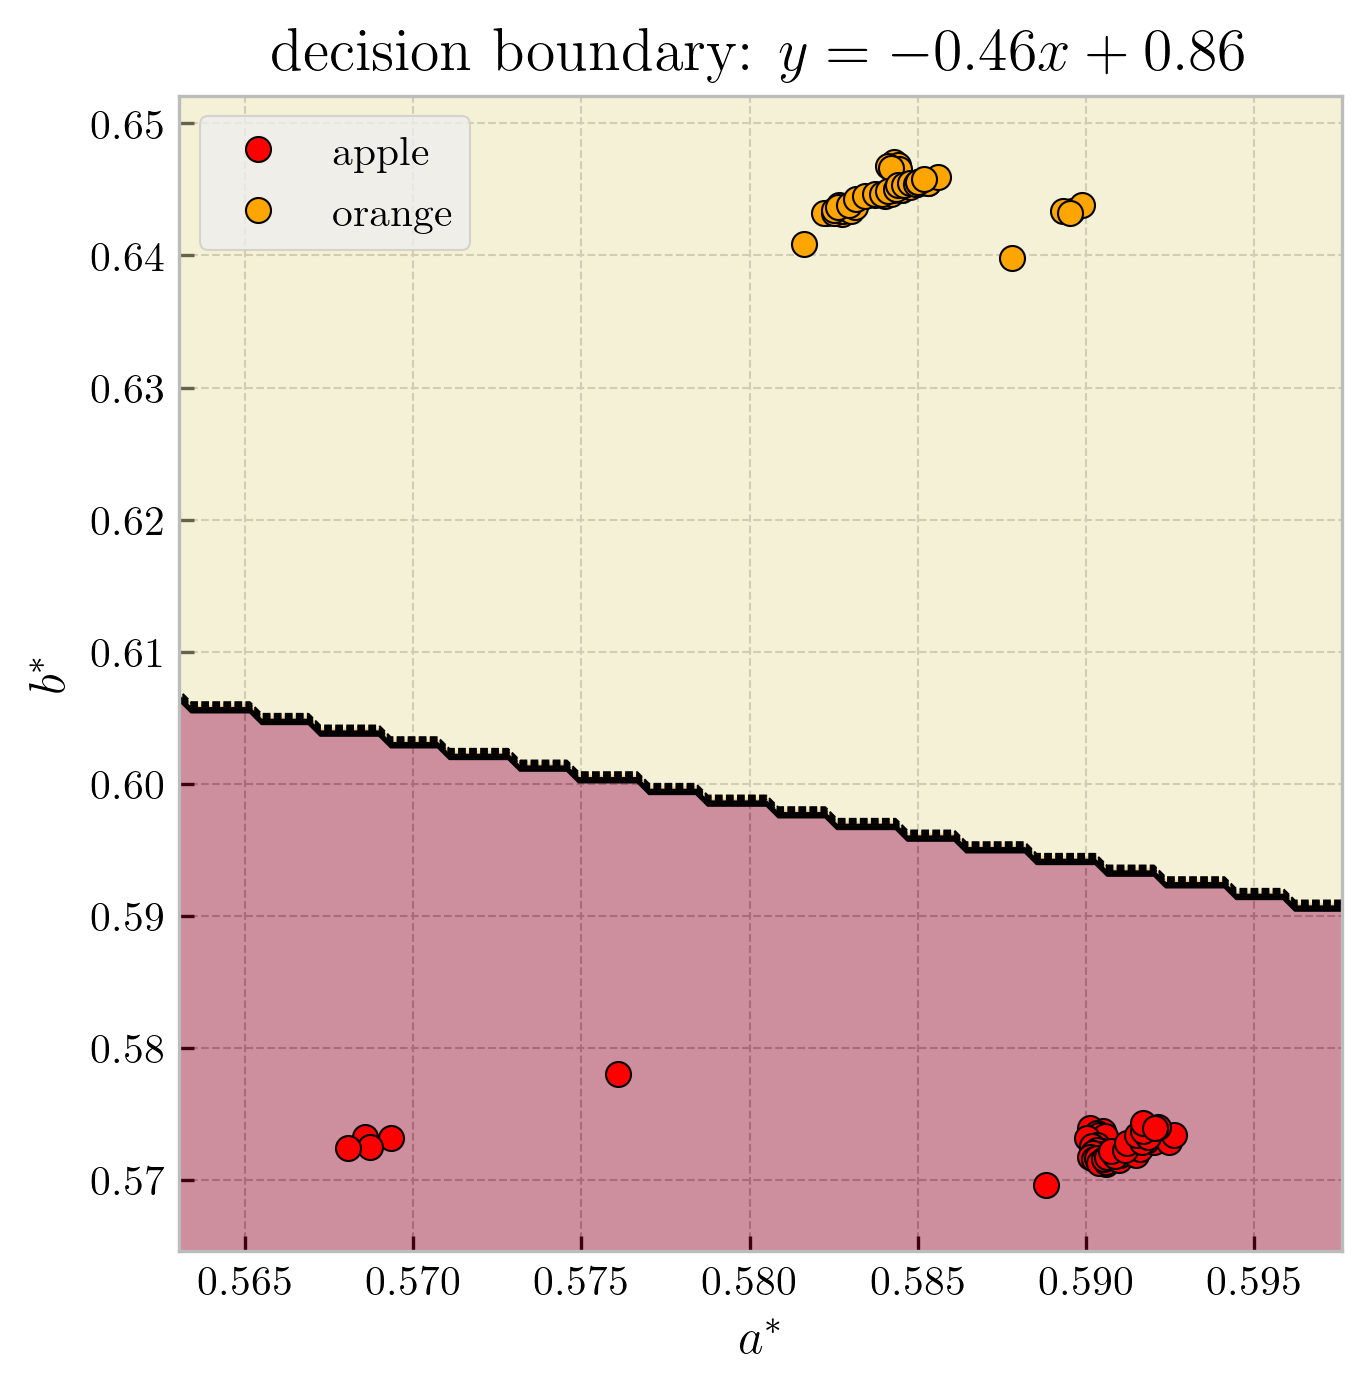
\includegraphics[width=\textwidth]{app-ora_decision.png}
		\caption{apple-orange}
		\label{fig:apple-orange}
	\end{subfigure}
	\caption{Decision boundaries for each class pair.}
	\label{fig:boundaries}
\end{figure}

%\clearpage
\begin{table}[!htb]
	\centering
	\caption{Self-evaluation.}
	\begin{tabular}{||r|c||}
		\hline
		Technical correctness & 5 \\ \hline
		Quality of presentation & 5 \\ \hline
		Initiative & 0 \\ \hline
		\textbf{TOTAL} & \textbf{10} \\ \hline
	\end{tabular}
	\label{tab:self-eval}
\end{table}

\bibliographystyle{spp-bst}
\bibliography{biblio}

\end{document}